\documentclass[dvipdfm,serif,mathserif]{beamer}
\usepackage{color}
\usepackage{amsmath, amsfonts, epsfig, xspace}
\usepackage{algorithm,algorithmic}
\usepackage{pstricks,pst-node}
\usepackage{multimedia}
\usepackage[normal,tight,center]{subfigure}
\usepackage[boldfont,slantfont,CJKnumber]{xeCJK}

\setCJKmainfont[BoldFont=Adobe Heiti Std]{Adobe Song Std} % 设置默认的中文字体
\setCJKfamilyfont{kai}{Adobe Kaiti Std}

\definecolor{darkgreen}{rgb}{0,.39,0}

\renewcommand{\today}{\number\year 年 \number\month 月 \number\day 日}
\usetheme{Singapore}

\definecolor{steelblue}{rgb}{.275,.51,.71}
\definecolor{lpink}{rgb}{.991,.711,.754}
\definecolor{mygray}{gray}{0.92}
\definecolor{darkblue}{rgb}{0,0,.5}
\definecolor{darkgreen}{rgb}{0,.39,0}
\definecolor{hgray}{gray}{.5}
\definecolor{lgray}{gray}{.8}

\graphicspath{{data/}} %%图片路径
%  \DeclareGraphicsExtensions{.}
\hypersetup{pdfpagemode={FullScreen}} % 全屏幕

\begin{document}

% \author{颜开}
\title{The First Talk of \textcolor{darkgreen}{iMath}}
\date{\today}
\author{Jerry Mouse}

\begin{frame}
  \titlepage
\end{frame}
\begin{frame}\frametitle{目录}
\tableofcontents
\end{frame}


\AtBeginSection[] {
  \frame<handout:0> {
    \frametitle{目录}
    \tableofcontents[current]
  }
}

\section{来点实际的}

\begin{frame}
  \frametitle{效果图}
  \begin{center}
  \includegraphics[width=\textwidth]{init1.1.ps}
 \end{center}
\end{frame}

\begin{frame}
  \frametitle{目标}
\begin{enumerate}
 \item 做同学老师满意的软件
 \item 与MathLab竞争市场
\end{enumerate}
\end{frame}

\section{流程}

\begin{frame}
  \frametitle{一期}
\begin{itemize}
 \item[时间] Now -  5月10日
 \item[框架] 马马虎虎作出框架,注重定义接口
 \item[工具] 基本工具要有,但不多
\end{itemize}
\end{frame}

\begin{frame}
  \frametitle{二期上}
\begin{itemize}
 \item[时间] 5月10日 - 5月20日
 \item[框架] 完善框架,注重美观
 \item[工具] 完善丰富工具集
\end{itemize}
\end{frame}

\begin{frame}
  \frametitle{二期下}
\begin{itemize}
 \item[时间] 5月20日 - 6月1日
 \item[框架] 完善框架,注重效果,用户体验
 \item[工具] 继续完善丰富工具集,出一个精品工具
\end{itemize}
\end{frame}

\section{技术}

\begin{frame}
  \frametitle{Apache Math}
\begin{minipage}[c]{0.6\textwidth}
\begin{itemize}
 \item 比较完整的统计包
 \item 数不清的工具包
 \item 文档很长很完整
\end{itemize}
  \end{minipage}
  \begin{minipage}[c]{0.3\textwidth}
  
\includegraphics[width=\textwidth]{math.ps}
  \end{minipage}
 \end{frame}

\begin{frame}
  \frametitle{JavaEE}
\begin{itemize}
 \item Maven:不错的构建工具
 \item Struts2
  \item Dojo
  \item Spring
   \item \color{darkblue}{CXF(Celtix/Xfire) or Axis2:Web Service}
\end{itemize}
\end{frame}

\begin{frame}
  \frametitle{Google相关}
\begin{itemize}
\begin{minipage}[c]{0.6\textwidth}
 \item Gears
 \item Google Chart API
 \item Google Gidget API
 \item \color{darkblue}{Google App Engine}
  \end{minipage}
  \begin{minipage}[c]{0.3\textwidth}
  
\includegraphics[width=\textwidth]{appengine_lowres.ps}
  \end{minipage}
\end{itemize}
\end{frame}

\section{做完以后}

\begin{frame}
  \frametitle{Beta Forever}
\begin{center}
 \begin{Large}  此是后话,不提
\end{Large} 

\end{center}

\end{frame}

\section{结语}

\begin{frame}
%   \frametitle{谢谢}
\begin{center}
 \begin{LARGE}88 \end{LARGE} 
\end{center}
\end{frame}
\end{document}
